\documentclass[12pt]{article} 
\usepackage[utf8]{inputenc} % ç etc
\usepackage[portuges]{babel} % portugues
\usepackage{amsmath} % pacote de equações
\usepackage{graphicx} % figuras
\usepackage{float}  % deal with figure position [H]
\usepackage{subcaption} % deal with subfigures
\graphicspath{{images/}} %configuring the graphicx package

\title{Exemplo de usos de LaTeX}
\author{Eu Mesmo}
\date{\today}
\begin{document}
\maketitle

% some formatting

Some of the \textbf{greatest}
discoveries in \underline{science} 
were made by \textbf{\textit{accident}}.


% adding images

% t: top of the page
% b: bottom of the page 

\begin{figure}[H] % places figure here. can use more than one.
    \centering
    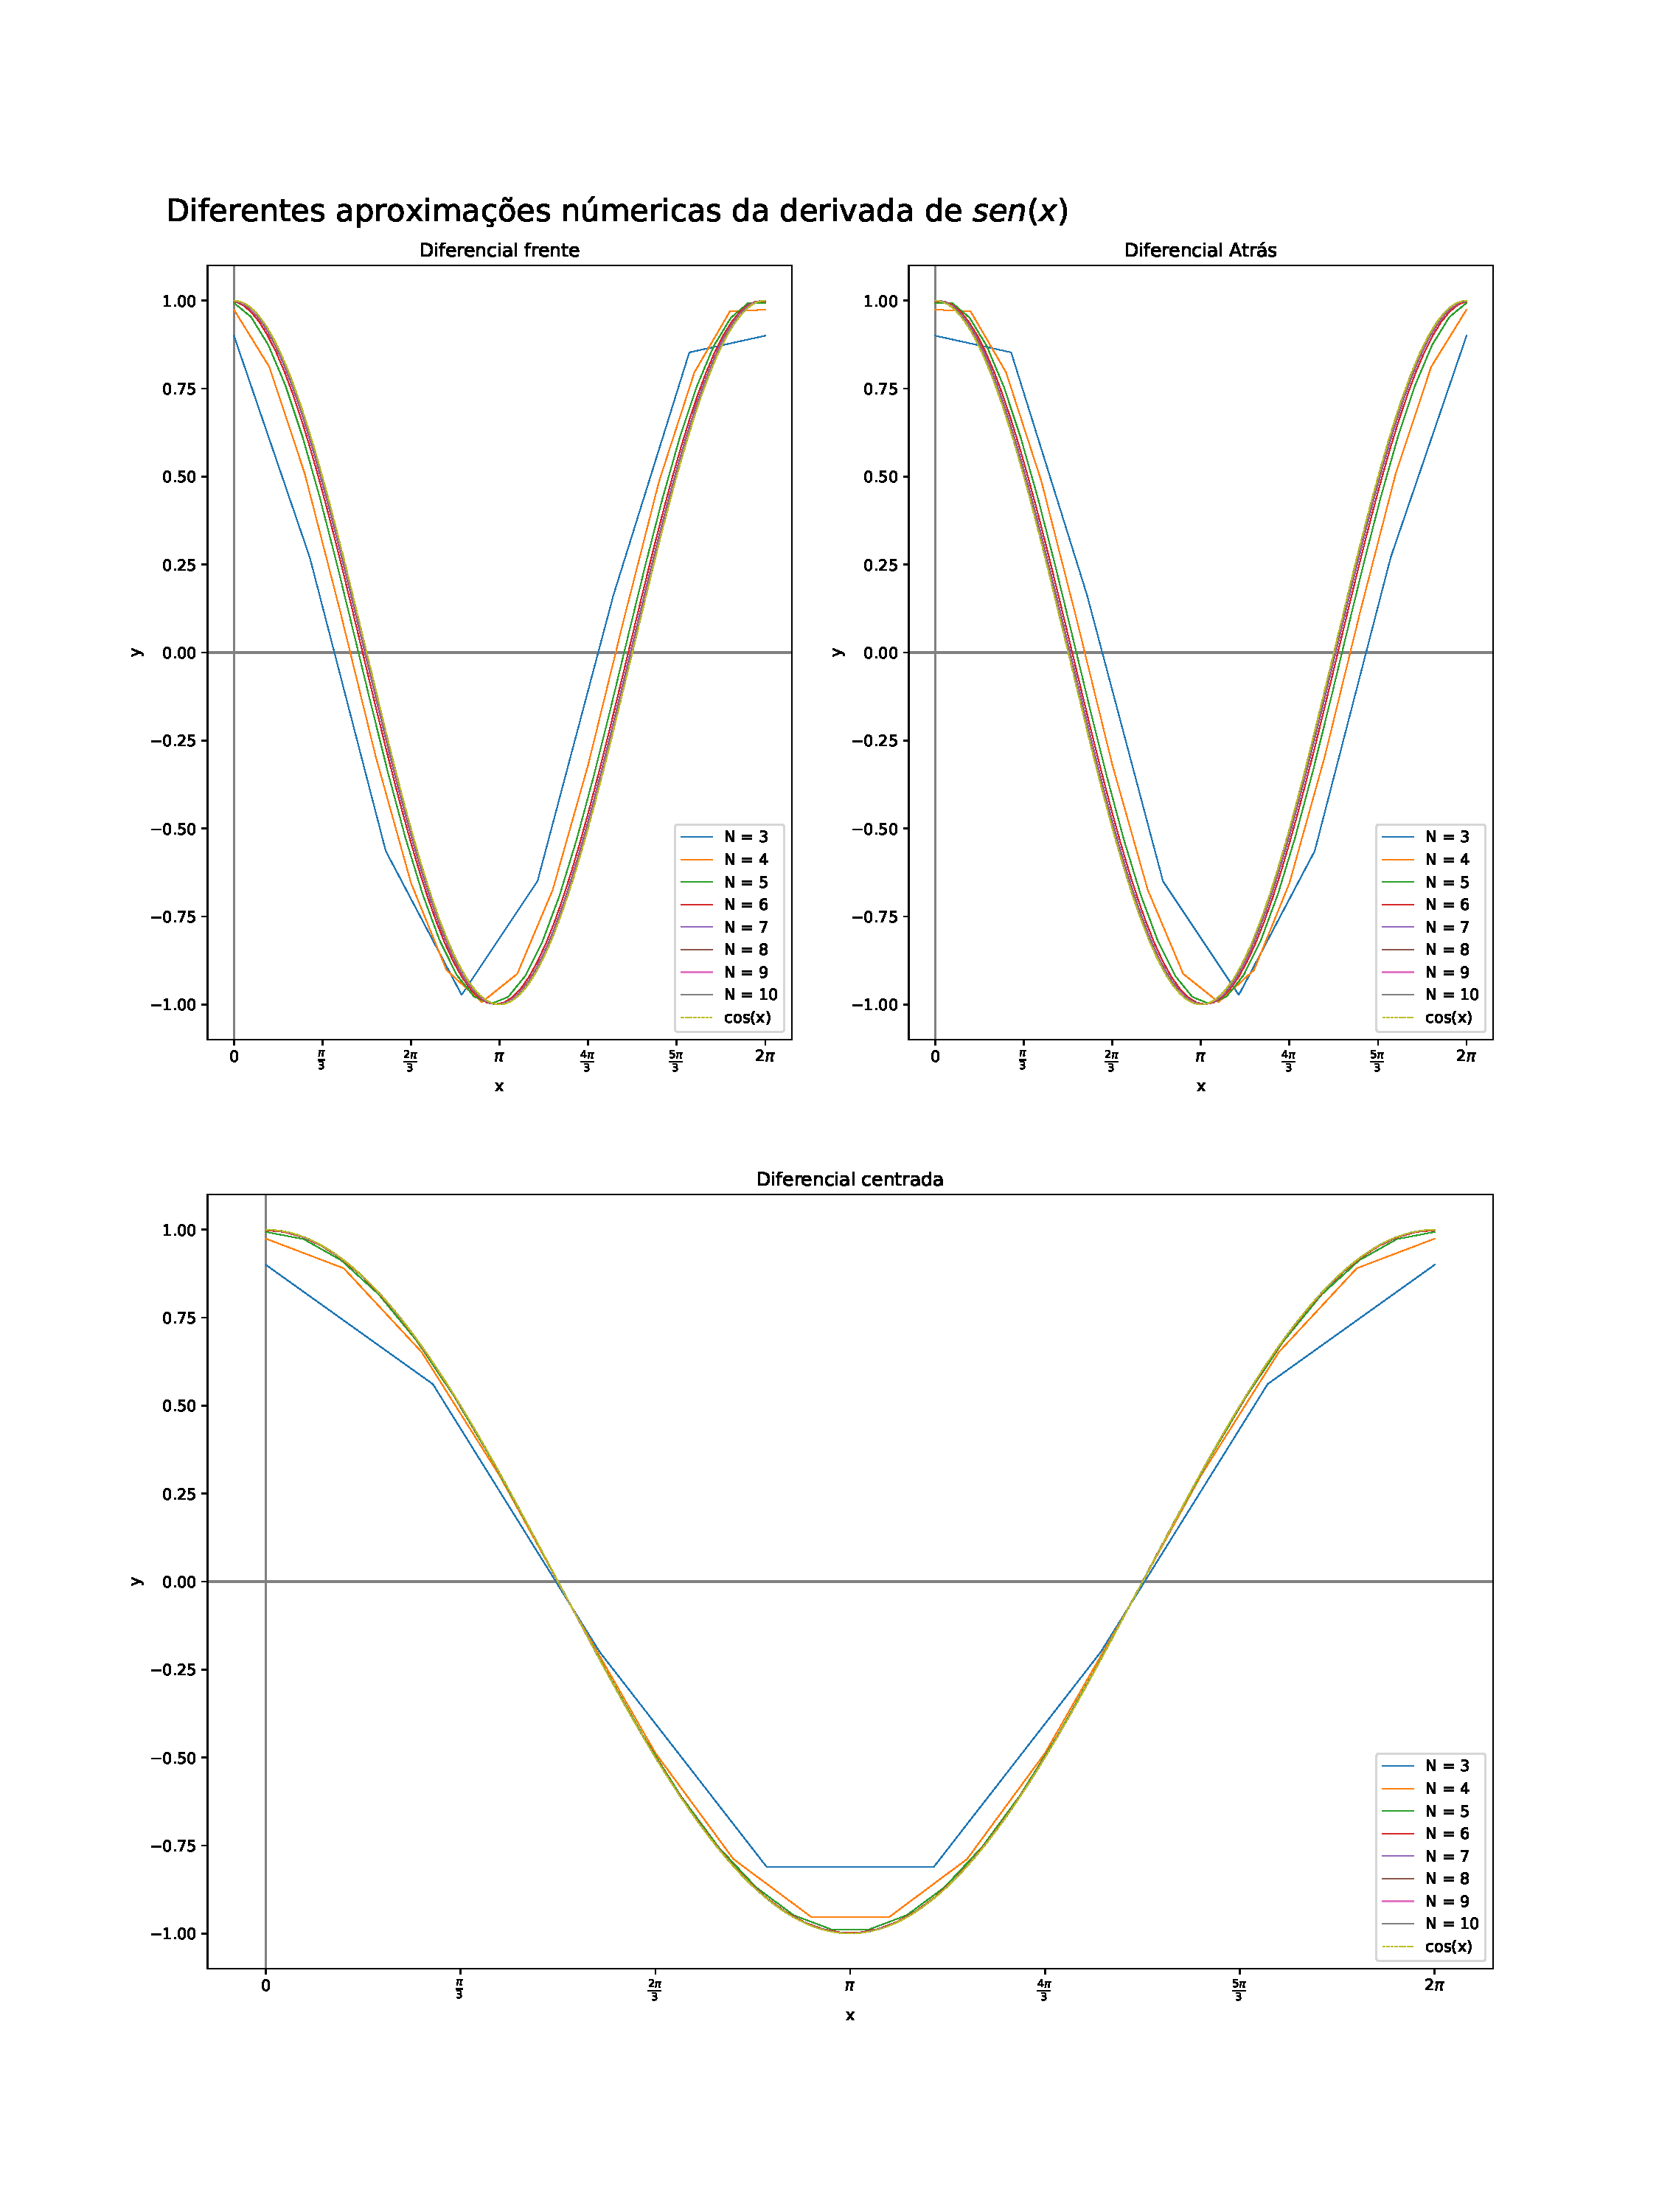
\includegraphics[width=0.9\linewidth]{derivadas.pdf}
    \caption{bonitao}
    \label{fig:derivadas}
\end{figure}
As you can see in figure \ref{fig:derivadas}, thats how you make a reference.

\begin{figure}[h]

\begin{subfigure}{0.5\textwidth}
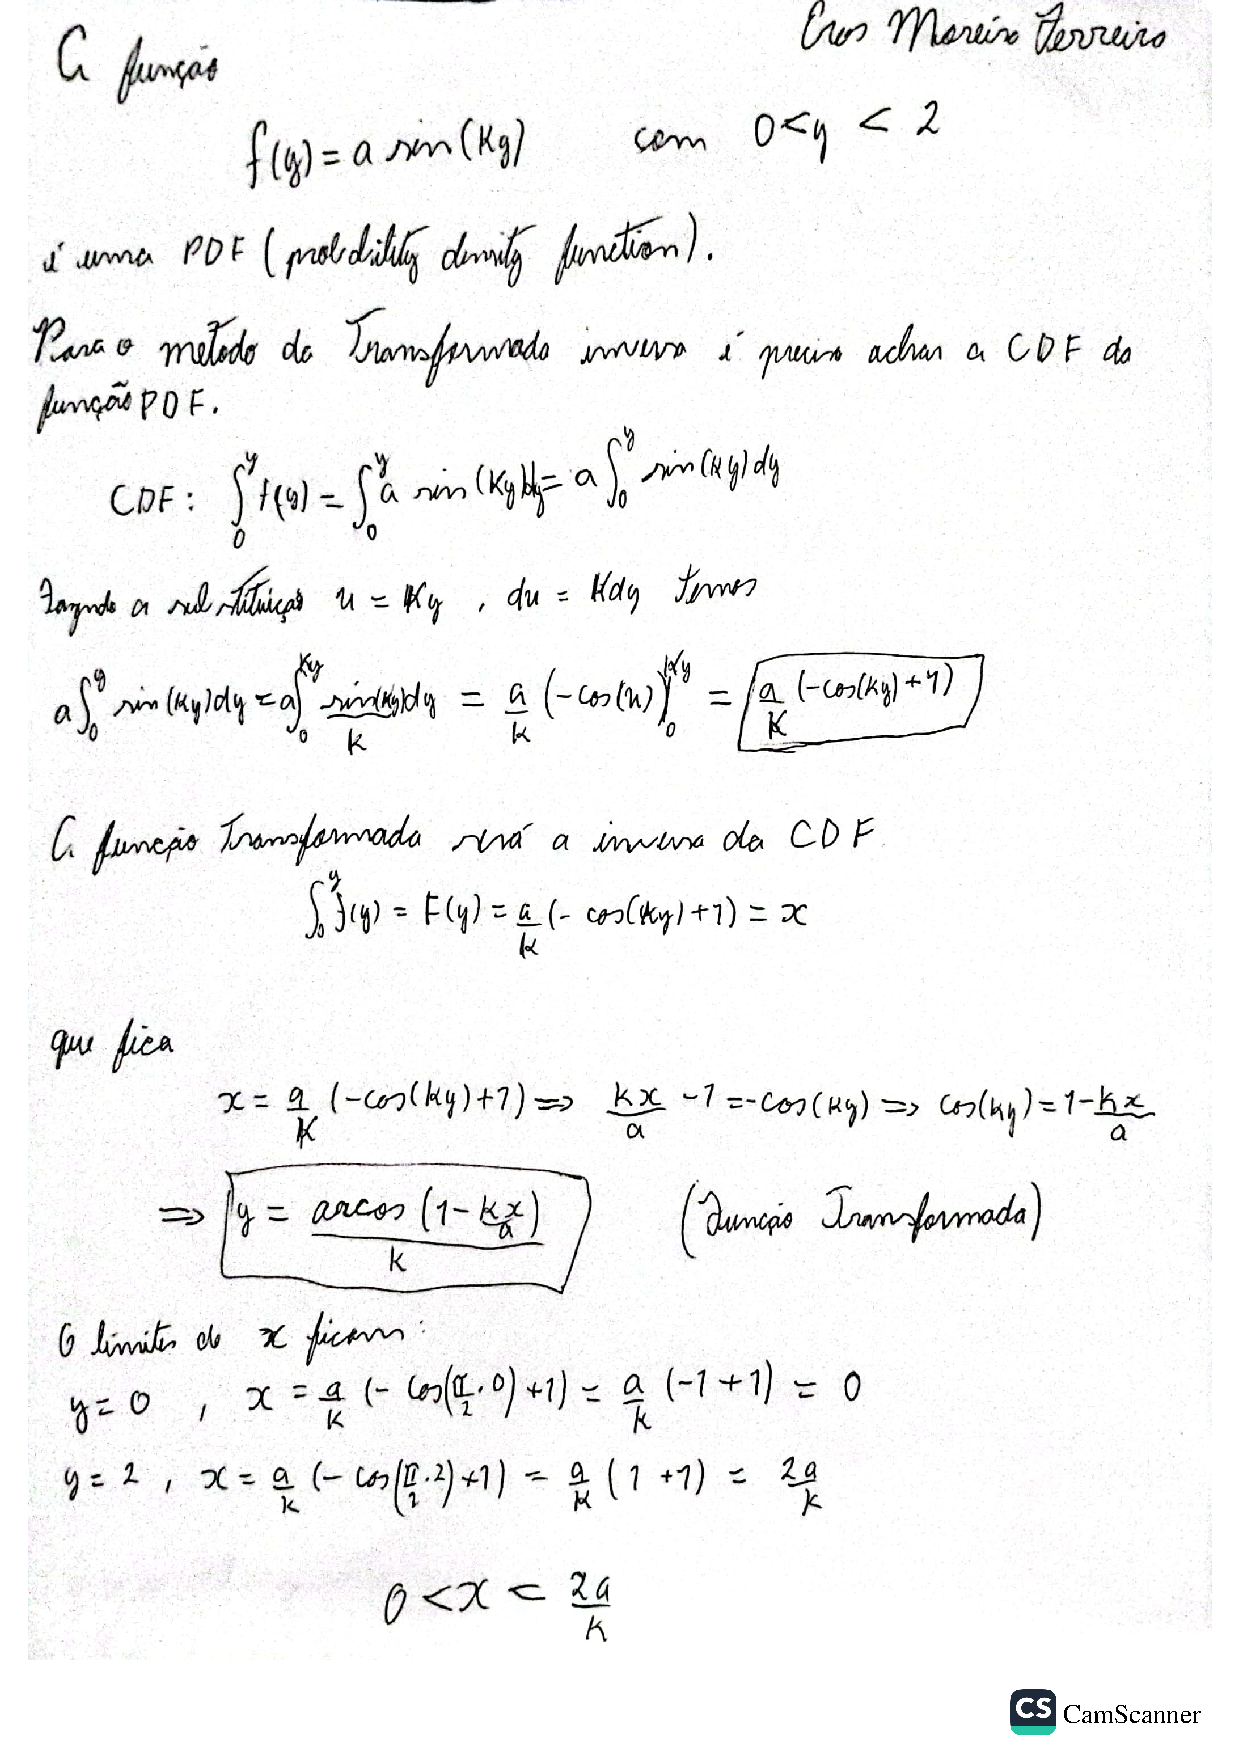
\includegraphics[width=0.9\linewidth]{transformada_inversa.pdf} 
\caption{Caption1}
\label{fig:subim1}
\end{subfigure}

\begin{subfigure}{0.5\textwidth}
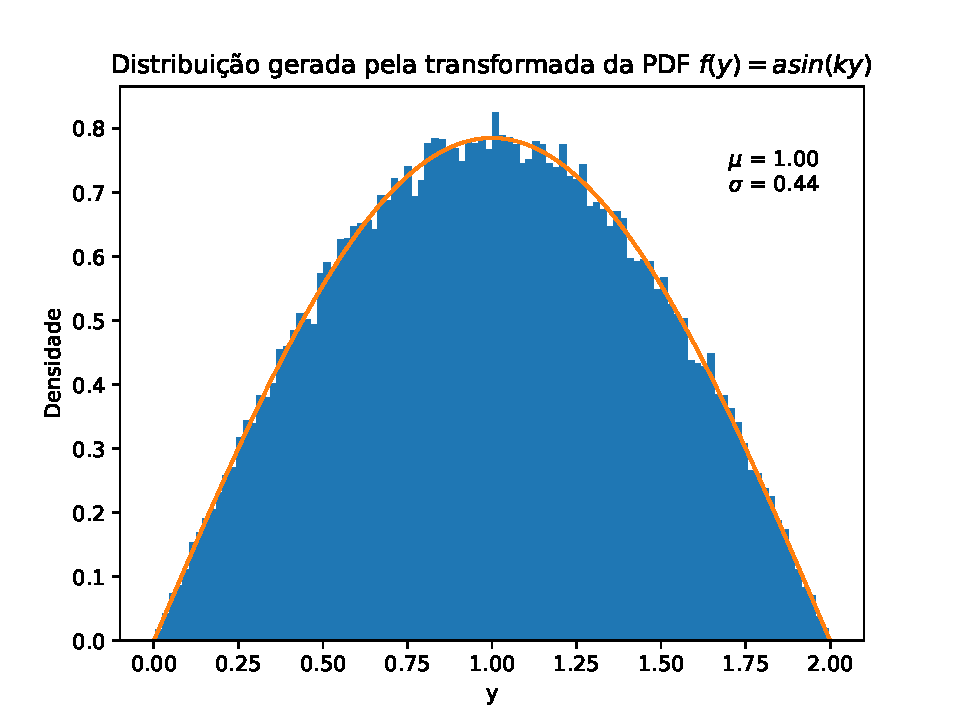
\includegraphics[width=0.9\linewidth]{transformada_seno.pdf}
\caption{Caption 2}
\label{fig:subim2}
\end{subfigure}

\caption{Caption for this figure with two images}
\label{fig:image2}
\end{figure}


% listas

AS listas são feitas assim.
\begin{itemize}
    \item item 1
    \item item 2
    \item item 3
\end{itemize}

ou

\begin{enumerate}
    \item item 1
    \item item 2
    \item item 3
\end{enumerate}


% add math


\begin{math}
    E=mc^2
\end{math}
is typeset in a paragraph using inline math mode---as is $E=mc^2$, and so too is \(E=mc^2\).

Equations typeset in display mode can be numbered or unnumbered, as in the following example:

The mass-energy equivalence is described by the famous equation
\[ E=mc^2 \] discovered in 1905 by Albert Einstein. 

In natural units ($c = 1$), the formula expresses the identity
\begin{equation}
E=                              % use equation when you want a numbered equation
\end{equation}

This is a simple math expression \(\sqrt{x^2+1}\) inside text. 
And this is also the same: 
\begin{math}
\sqrt{x^2+1}
\end{math}
but by using another command.

\[ x^n + y^n = z^n \]


This is a simple math expression without numbering
\[\sqrt{x^2+1}\] 
separated from text.

This is also the same:
\begin{displaymath}
\sqrt{x^2+1}
\end{displaymath}

\end{document} 